\subsection{Supplementary figures and text}

\begin{figure}
    \begin{center}
      \includegraphics{../illustrations/parameter_estimation_scheme.pdf}
    \end{center}
    \caption{Scheme of parameter estimation method. Values for the rate
    constant of NAC, promoter escape, and unscrunching and abortive release
    are randomly sampled. The value for NAC and the promoter APs are used to
    obtain the rate constant for backstepping. The four rate constants are
    used to simulate 100 initial transcription events. The time-distribution
    of scrunching from the simulations are compared with experimental data.}
    \label{fig:parameter_estimation_scheme}
\end{figure}

\begin{figure}
    \begin{center}
        \includegraphics{../figures/aps_after_adjustment.pdf}
    \end{center}
    \caption{Modified APs from the +GreB baseline. When negative APs were
    obtained, a value of 0 was used.}
    \label{fig:aps_after_adjustment}
\end{figure}
